\documentclass[11pt,letterpaper]{refart}

\usepackage{gitinfo2}
\usepackage{amsmath,mathtools}

\usepackage{hyperref}
\usepackage{cleveref}
\usepackage{caption}

\usepackage{microtype}
\usepackage[T1]{fontenc}

\usepackage{graphicx}
\usepackage{framed}
\usepackage{tikz}
\usepackage{booktabs}

\usepackage{xcolor}
\usepackage{listings}
\lstset{
    basicstyle=\ttfamily\footnotesize,
    breaklines=true,
    postbreak=\mbox{\textcolor{red}{$\hookrightarrow$}\space},
    frame=single,
    columns=flexible
}

% Figures can only float within its *subsection*
\usepackage{placeins}
\makeatletter
\AtBeginDocument{%
    \expandafter\renewcommand\expandafter\subsection\expandafter
        {\expandafter\@fb@secFB\subsection}%
    \expandafter\renewcommand\expandafter\section\expandafter
        {\expandafter\@fb@secFB\section}%
    \newcommand\@fb@secFB{\FloatBarrier
        \gdef\@fb@afterHHook{\@fb@topbarrier \gdef\@fb@afterHHook{}}}%
    \g@addto@macro\@afterheading{\@fb@afterHHook}%
        \gdef\@fb@afterHHook{}%
}%
\makeatother

\usepackage{chngcntr}
\counterwithin{figure}{subsection}

% For FAQ
\newcounter{question}
\setcounter{question}{0}
\newcounter{answer}
\setcounter{answer}{0}

\newcommand\Que[1]{%
   \stepcounter{question}%
   \noindent%
   \par\textbf{Q\thequestion.} \emph{#1}}\par%

\newcommand\Ans[1]{%
    \stepcounter{answer}%
    \noindent%
    \par\textbf{A\theanswer.} #1}\par%

% Better typesetted 'I2C'
\def\itwoc{I{$\scriptstyle^2$}C\ }
\newcommand\symbolwithin[2]{%
    {\mathmakebox[\widthof{\ensuremath{{}#2{}}}][c]{{#1}}}}

\title{GBTx Boards Documentation}
\author{University of Maryland LHCb group}

\begin{document}
\maketitle
\hfill\small{\texttt{Rev:~\gitRel~(\gitAbbrevHash)}}
\tableofcontents
\listoffigures
\clearpage

\section{Safety}
Safety is the most important thing in a lab. Please follow institutional guidelines.
In addition, the MiniDAQ server uses standard 110 V AC power. Please be careful
when handling this voltage.
The MiniDAQ server is also heavy, when removing it from the rack at least two
persons are needed and must proceed with caution.

To make sure no board is damaged accidentally, please:
\begin{itemize}
    \item Always wear ESD-safe straps.
    \item Place all boards on an ESD-safe desktop.
    \item Handle the board with caution to avoid dropping.
    \item Install connectors gently to avoid bending or damaging them.
    \item When disconnecting components it is preferable to wiggle them parallel
        to the long axis rather than the short axis of the pinout.
    \item Always double check the power supply output parameter before turn them
        on or connect them to boards. Make sure these parameters are correct.
\end{itemize}


\section{Setup data control board}
\subsubsection{Overview}
Data control board (DCB) are intented to be a part of the LHCb upstream tracker
upgrade.
There is one master GBTx ASIC, and 6 data GBTx ASICs per board.
DCB is much less flexible than GBTx DB, because it serves only one purpose:
Receive SALT elink data then transmit that data to the counting room.

So far, we have been able to repeat PRBS test on DCBs:
Programming the master, then programming data GBTxs, then instruct them to
generate PRBS data, and verify generated data by MiniDAQ.

\autoref{fig:dcb_layout} shows the layout of an actual DCB board.
%GBTx ASICs layout are marked on the figure directly.
Optical fiber grouping are marked by the \texttt{OMDBXX} label. For example,
\texttt{OMDB23} means that data GBTxs 2 and 3 are connected to this mezzanine.

A DCB requires 4 optical mezzanines (not shown here) to function properly.
As said above, DCB is less flexible, and there will be only \emph{one}
configuration for DCBs.
All DCBs shipped by UMD LHCb group will have its hardware jumpers
pre-configured.

\begin{figure}[!ht]
\centering
\begin{tikzpicture}
    \node [anchor=south west] (main) {
            \includegraphics[width=0.9\linewidth]{res/dcb_layout.png}
        };
    \begin{scope}[x=(main.south east),y=(main.north west)]
        \draw [fill=none,red,very thick] (0.24,0.76) rectangle ++(0.0813,0.1)
            node [pos=.5] {\tiny\texttt{data 1}};
        \draw [fill=none,red,very thick] (0.24,0.135) rectangle ++(0.0813,0.1)
            node [pos=.5] {\tiny\texttt{data 6}};

        \draw [fill=none,blue,very thick] (0.49,0.76) rectangle ++(0.0813,0.1)
            node [pos=.5] {\tiny\texttt{data 2}};
        \draw [fill=none,blue,very thick] (0.74,0.76) rectangle ++(0.0813,0.1)
            node [pos=.5] {\tiny\texttt{data 3}};

        \draw [fill=none,cyan,very thick] (0.74,0.135)
                rectangle ++(0.0813,0.1)
            node [pos=.5] {\tiny\texttt{data 4}};
        \draw [fill=none,cyan,very thick] (0.49,0.135)
                rectangle ++(0.0813,0.1)
            node [pos=.5] {\tiny\texttt{data 5}};

        \draw [fill=none,orange,very thick] (0.74,0.448) rectangle ++(0.0813,0.1)
            node [pos=.5] {\tiny\texttt{master}};

        \draw [fill=none,magenta,very thick] (0.77,0.88) rectangle ++(0.17,0.05)
            node [pos=.5] {\tiny\texttt{power}};
    \end{scope}
\end{tikzpicture}
\caption{Pilot-run DCB layout.}
\label{fig:dcb_layout}
\end{figure}

\subsubsection{Power DCB without backplane}

\subsubsection{Prepare FFC cable}
To use FFC breakout board for debugging, FFC cables with ground shielding should
be purchased.

If normal FFC cables (it seems that, at least in the U.S., it is harder to find
properly-shielded FFC cables) are purchased, an additional manual modification
needs to be done on the optical mezzanine side of the cable connector:
A insulation tape (possibly Kapton tape) should be applied on the lower 1/4 of
the connector, so that the shielding pins on the optical mezzanine are masked
(ineffective).
See \autoref{fig:ffc-cable} for FFC breakout cable with modification.

\begin{figure}[!ht]
    \centering
    \includegraphics[width=0.9\linewidth]{res/ffc_breakout_cable_with_tape.jpg}
    \caption{FFC breakout cable with modification.}
    \label{fig:ffc-cable}
\end{figure}

\begin{leftbar}
    Note that after prolonged use, the metal contact pin may penetrate the
    Kapton tape on the FFC cable connector, rendering the trick shown in
    \autoref{fig:ffc-cable} ineffective.

    To fix the problem, redo the trick;
    alternatively, trim the FFC cable connector to make it shorter---this should
    be a more permanent solution.
\end{leftbar}

\subsubsection{Configure GBTx DB to use external \itwoc adapter}
A FFC breakout board is needed to connect \itwoc adapter to the DCB GBTx master.
Follow \autoref{fig:dcb_mc_i2c} to connect an external \itwoc adapter.

\begin{figure}[!ht]
\centering
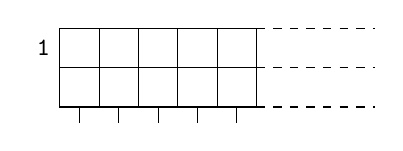
\begin{tikzpicture}
    % Pins
    \draw (0,0) rectangle (0.5,0.5);
    \draw (0.5,0) rectangle (1,0.5);
    \draw (1,0) rectangle (1.5,0.5);
    \draw (1.5,0) rectangle (2,0.5);
    \draw (2,0) rectangle (2.5,0.5);

    \draw (0,-0.5) rectangle (0.5,0);
    \draw (0.5,-0.5) rectangle (1,0);
    \draw (1,-0.5) rectangle (1.5,0);
    \draw (1.5,-0.5) rectangle (2,0);
    \draw (2,-0.5) rectangle (2.5,0);

    % Extension lines
    \draw [dashed] (2.5,0.5) -- (4,0.5);
    \draw [dashed] (2.5,0) -- (4,0);
    \draw [dashed] (2.5,-0.5) -- (4,-0.5);

    % Additional copper traces
    \draw (0.25,-0.5) -- (0.25,-0.7);
    \draw (0.75,-0.5) -- (0.75,-0.7);
    \draw (1.25,-0.5) -- (1.25,-0.7);
    \draw (1.75,-0.5) -- (1.75,-0.7);
    \draw (2.25,-0.5) -- (2.25,-0.7);

    % Helper labels (imaginary)
    \coordinate (B) at (0,0.25);
    \node at (B) [left] {\small\texttt{1}};

    % Single cable on the I2C
    %\draw [black,fill] (0.25,0.25) circle [radius=0.1];
    %\draw [thick] (0.25,0.25)
        %to [out=10,in=190] (5,-1) node [right]
        %{To single cable};

    %% 2x1 connector on the I2C
    %\draw [black,fill] (0.25,-0.25) circle [radius=0.1];
    %\draw [black,fill] (0.75,-0.25) circle [radius=0.1];
    %\draw [thick] (0.25,-0.25) to [out=-80,in=120] (1,-1);
    %\draw [thick] (0.75,-0.25) to [out=-90,in=130] (1,-1);
    %\draw [thick] (1,-1)
        %to [out=-50,in=170] (5,-2) node [right]
        %{To 2x1 connector};
\end{tikzpicture}
\caption{Schematic for external \itwoc adapter setup.}
\label{fig:dcb_mc_i2c}
\end{figure}

\subsection{Connect \itwoc adapter to DCB data GBTxs}
\label{sec:dcb-data-i2c}
\itwoc adapter can be connected to the DCB mainboard directly, so that all 6
data GBTxs can be accessed via \itwoc.
Note that a FFC breakout board \emph{is still required} in this case, as no
ground connector is present on the mainboard and must be connected to any of the
4 FFC breakout boards.
Follow \autoref{fig:dcb-data-i2c} to connect an external \itwoc
adapter\footnote{
    As a reminder, in UMD, \itwoc adapter color coding is:
    yellow $\rightarrow$ \texttt{I2C SCL};
    blue $\rightarrow$ \texttt{I2C SDA};
}.

\begin{figure}[!ht]
\centering
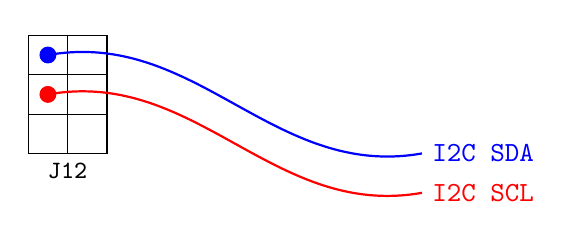
\begin{tikzpicture}
    % Pins
    \draw (0,0) rectangle (0.5,0.5);
    \draw (0.5,0) rectangle (1,0.5);

    \draw (0,-0.5) rectangle (0.5,0);
    \draw (0.5,-0.5) rectangle (1,0);

    \draw (0,-1) rectangle (0.5,-0.5);
    \draw (0.5,-1) rectangle (1,-0.5);

    % Helper labels (imaginary)
    \coordinate (B) at (0.5,-1);
    \node at (B) [below] {\small\texttt{J12}};

    % I2C SCL
    \draw [red,fill] (0.25,-0.25) circle [radius=0.1];
    \draw [red,thick] (0.25,-0.25)
        to [out=10,in=190] (5,-1.5) node [right] {\texttt{I2C SCL}};

    % I2C SDA
    \draw [blue,fill] (0.25,0.25) circle [radius=0.1];
    \draw [blue,thick] (0.25,0.25)
        to [out=10,in=190] (5,-1) node [right] {\texttt{I2C SDA}};
\end{tikzpicture}
\caption{
    \itwoc adapter can be connected on the DCB mainboard to access all 6 data
    GBTxs.
    Also note that no \texttt{GND} is present thus FFC breakout board is still
    required.
}
\label{fig:dcb-data-i2c}
\end{figure}

\subsubsection{Reset DCB master GBTx}
A hardware reset can be performed on the master FFC breakout board to reset the
master GBTx (See \autoref{fig:dcb_mc_reset}).

\begin{figure}[!ht]
\centering
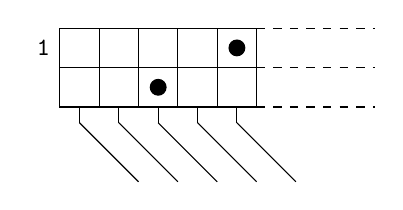
\begin{tikzpicture}
    % Pins
    \draw (0,0) rectangle (0.5,0.5);
    \draw (0.5,0) rectangle (1,0.5);
    \draw (1,0) rectangle (1.5,0.5);
    \draw (1.5,0) rectangle (2,0.5);
    \draw (2,0) rectangle (2.5,0.5);

    \draw (0,-0.5) rectangle (0.5,0);
    \draw (0.5,-0.5) rectangle (1,0);
    \draw (1,-0.5) rectangle (1.5,0);
    \draw (1.5,-0.5) rectangle (2,0);
    \draw (2,-0.5) rectangle (2.5,0);

    % Extension lines
    \draw [dashed] (2.5,0.5) -- (4,0.5);
    \draw [dashed] (2.5,0) -- (4,0);
    \draw [dashed] (2.5,-0.5) -- (4,-0.5);

    % Additional copper traces
    \draw (0.25,-0.5) -- (0.25,-0.7);
    \draw (0.75,-0.5) -- (0.75,-0.7);
    \draw (1.25,-0.5) -- (1.25,-0.7);
    \draw (1.75,-0.5) -- (1.75,-0.7);
    \draw (2.25,-0.5) -- (2.25,-0.7);

    \draw (0.25,-0.7) -- (1,-1.45);
    \draw (0.75,-0.7) -- (1.5,-1.45);
    \draw (1.25,-0.7) -- (2,-1.45);
    \draw (1.75,-0.7) -- (2.5,-1.45);
    \draw (2.25,-0.7) -- (3,-1.45);

    % Helper labels (imaginary)
    \coordinate (B) at (0,0.25);
    \node at (B) [left] {\small\texttt{1}};

    % GND
    \draw [black,fill] (2.25,0.25) circle [radius=0.1];

    % RESET
    \draw [black,fill] (1.25,-0.25) circle [radius=0.1];
\end{tikzpicture}
\caption{
    Connect the two pins marked above with a jumper/wire to reset DCB master
    GBTx.
    Note that pin 7 and 9 are both \texttt{GND}.
}
\label{fig:dcb_mc_reset}
\end{figure}

\subsubsection{Manually pull up \texttt{TX\_DATAVALID}}
DCB pilot boards do not have pull-up resistor to pull up \texttt{TX\_DATAVALID}
automatically.
This would prevent PRBS tests, since without it pulling up, MiniDAQ would
consider data frames as ``invalid''\footnote{
    Which is not really the case, as all \texttt{TX\_DATAVALID} does is flip
    single bit 0 to 1 on the header part of the data frame.
}.

A large ($\approx$ 5~k$\Omega$) resistor is connected between the \emph{data
GBTx} FFC breakout board \texttt{TX\_DATAVALID} pin and 1.5~V rail.
See \autoref{fig:dcb_tx_datavalid_pull_up} for connection details.

\begin{figure}[!ht]
\centering
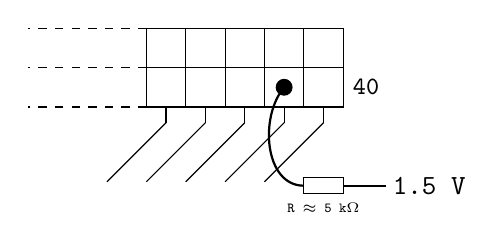
\begin{tikzpicture}
    % Pins
    \draw (0,0) rectangle (0.5,0.5);
    \draw (0.5,0) rectangle (1,0.5);
    \draw (1,0) rectangle (1.5,0.5);
    \draw (1.5,0) rectangle (2,0.5);
    \draw (2,0) rectangle (2.5,0.5);

    \draw (0,-0.5) rectangle (0.5,0);
    \draw (0.5,-0.5) rectangle (1,0);
    \draw (1,-0.5) rectangle (1.5,0);
    \draw (1.5,-0.5) rectangle (2,0);
    \draw (2,-0.5) rectangle (2.5,0);

    % Extension lines
    \draw [dashed] (0,0.5) -- (-1.5,0.5);
    \draw [dashed] (0,0) -- (-1.5,0);
    \draw [dashed] (0,-0.5) -- (-1.5,-0.5);

    % Additional copper traces
    \draw (0.25,-0.5) -- (0.25,-0.7);
    \draw (0.75,-0.5) -- (0.75,-0.7);
    \draw (1.25,-0.5) -- (1.25,-0.7);
    \draw (1.75,-0.5) -- (1.75,-0.7);
    \draw (2.25,-0.5) -- (2.25,-0.7);

    \draw (0.25,-0.7) -- (-0.5,-1.45);
    \draw (0.75,-0.7) -- (0,-1.45);
    \draw (1.25,-0.7) -- (0.5,-1.45);
    \draw (1.75,-0.7) -- (1,-1.45);
    \draw (2.25,-0.7) -- (1.5,-1.45);

    % Helper labels (imaginary)
    \coordinate (B) at (2.5,-0.25);
    \node at (B) [right] {\small\texttt{40}};

    % TX_DATAVALID pin
    \draw [black,fill] (1.75,-0.25) circle [radius=0.1];
    \draw [black,thick] (1.75,-0.25) to [out=-130,in=180] (2,-1.5) node {};
    \draw (2,-1.4) rectangle (2.5,-1.6);
    \draw [black,thick] (2.5,-1.5) to [out=0,in=0] (3,-1.5)
        node [right] {\texttt{1.5~V}};

    % Resistor label
    \coordinate (A) at (2.25,-1.6);
    \node at (A) [below] {\tiny\texttt{R $\approx$ 5~k$\Omega$}};
\end{tikzpicture}
\caption{
    Manually pull up \texttt{TX\_DATAVALID} with a large resistor connected to
    1.5~V rail.
    Pay attention to the orientation of the FFC breakout board.
}
\label{fig:dcb_tx_datavalid_pull_up}
\end{figure}

An easier to implement, but not recommended way is listed in
\autoref{fig:dcb_tx_datavalid_pull_up_alt}.

\begin{figure}[!ht]
\centering
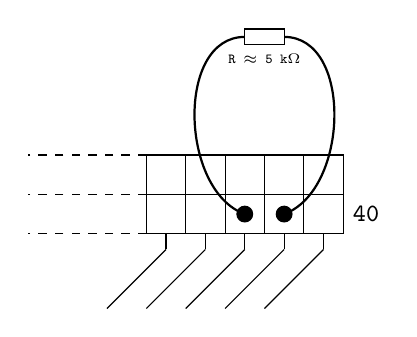
\begin{tikzpicture}
    % Pins
    \draw (0,0) rectangle (0.5,0.5);
    \draw (0.5,0) rectangle (1,0.5);
    \draw (1,0) rectangle (1.5,0.5);
    \draw (1.5,0) rectangle (2,0.5);
    \draw (2,0) rectangle (2.5,0.5);

    \draw (0,-0.5) rectangle (0.5,0);
    \draw (0.5,-0.5) rectangle (1,0);
    \draw (1,-0.5) rectangle (1.5,0);
    \draw (1.5,-0.5) rectangle (2,0);
    \draw (2,-0.5) rectangle (2.5,0);

    % Extension lines
    \draw [dashed] (0,0.5) -- (-1.5,0.5);
    \draw [dashed] (0,0) -- (-1.5,0);
    \draw [dashed] (0,-0.5) -- (-1.5,-0.5);

    % Additional copper traces
    \draw (0.25,-0.5) -- (0.25,-0.7);
    \draw (0.75,-0.5) -- (0.75,-0.7);
    \draw (1.25,-0.5) -- (1.25,-0.7);
    \draw (1.75,-0.5) -- (1.75,-0.7);
    \draw (2.25,-0.5) -- (2.25,-0.7);

    \draw (0.25,-0.7) -- (-0.5,-1.45);
    \draw (0.75,-0.7) -- (0,-1.45);
    \draw (1.25,-0.7) -- (0.5,-1.45);
    \draw (1.75,-0.7) -- (1,-1.45);
    \draw (2.25,-0.7) -- (1.5,-1.45);

    % Helper labels (imaginary)
    \coordinate (B) at (2.5,-0.25);
    \node at (B) [right] {\small\texttt{40}};

    % TX_DATAVALID pin and TX_RDY pin
    \draw [black,fill] (1.25,-0.25) circle [radius=0.1];
    \draw [black,fill] (1.75,-0.25) circle [radius=0.1];

    % Pull-up resistor, and its connection
    \draw (1.25,1.9) rectangle (1.75,2.1);
    \draw [black,thick] (1.25,-0.25) to [out=160,in=180] (1.25,2) node {};
    \draw [black,thick] (1.75,2) to [out=0,in=20] (1.75,-0.25) node {};

    % Resistor label
    \coordinate (A) at (1.5,1.9);
    \node at (A) [below] {\tiny\texttt{R $\approx$ 5 k$\Omega$}};
\end{tikzpicture}
\caption{
    Manually pull up \texttt{TX\_DATAVALID} with a large resistor.
    Here we are lazy, because we are using \texttt{TX\_RDY} to provide 1.5 V.
    This is strictly not recommended, but it works, and it creates less clutter
    in the setup.
    Pay attention to the orientation of the FFC breakout board.
}
\label{fig:dcb_tx_datavalid_pull_up_alt}
\end{figure}



\section{Software setup}
\subsection{Program master GBTx with external \itwoc adapter}
Before proceed, for GBTx DB, follow the instruction on
\autoref{sec:hardware-ext-i2c} to configure the hardware;
for DCB, connect \itwoc adapter to the GBTx master FFC breakout board, or DCB
mainboard as described on \autoref{sec:dcb-master-i2c} or
\autoref{sec:dcb-data-i2c}.

All GBTx configuration files are publicly available at
\url{https://github.com/ypsun-umd/gbtx_communication_doc/releases}.
Always use latest release.

It is recommended to use latest version of \textbf{GBTX programmer} provided by
CERN\footnote{
    Latest release can be found in CERN gitlab:
    \url{https://gitlab.cern.ch/gbtproj/gbtxprogrammer/tree/master/releases}.
    CERN credential needed to access the content.
}.

\begin{figure}[!ht]
    \centering
    \includegraphics[width=0.9\textwidth]{res/gbtx_programmer_v3_ui.png}
    \caption{Main UI of GBTX programmer, version 3.}
    \label{fig:gbtx-programmer-ui}
\end{figure}

Click \textbf{Import image} and load a configuration file, then click
\textbf{Write GBTX} to write to master GBTx via \itwoc.

\begin{leftbar}
    During DCB pilot testing, at least one DCB cannot be programmed by the
    latest version of GBTX Programer: It would stuck in state 10.
    In that case, please revert back to GBTX Programer v1.
\end{leftbar}

\begin{figure}[!ht]
    \centering
    \includegraphics[width=0.9\textwidth]{res/gbtx_programmer_v1_ui.png}
    \caption{Main UI of GBTX programmer, version 1.}
    \label{fig:gbtx-programmer-ui}
\end{figure}

Launch the programmer, a typical UI is shown in
\autoref{fig:gbtx-programmer-ui},
Click \textbf{Load GBTX configuration} and load a configuration file, which is

Then click \textbf{Write ALL to the GBTX}. Check the returned message to make
sure everything works (supposedly).
Now click \textbf{Read state}.
If the master GBTx is configured correctly and is connected to a working
MiniDAQ, the return value should be:

\begin{lstlisting}
24 (dec): Idle (normal status when running)
\end{lstlisting}

\input{include/software/check_communication_between_gbtx_and_minidaq.tex}
\subsection{Program slave GBTx with configuration files}
For slave (data) GBTxs, configuration filename should start with \texttt{slave}.
Typically, \texttt{slave-Tx.txt} is used.
Configure the parameter as shown in \autoref{fig:gbt-file}.

\begin{figure}[ht]
	\centering
    \includegraphics[width=0.9\textwidth]{res/gbt_client_slave_program_via_config_file.png}
	\caption{Parameters to program slave GBTx with a configuration file.}
	\label{fig:gbt-file}
\end{figure}

The configuration file should be supplied to the \textbf{Data in} field with the
following syntax:

\begin{lstlisting}
file:<path_to_configuration_file>
\end{lstlisting}

\begin{leftbar}
    This is equivalent to program the slave with an external \itwoc adapter.
    The advantage of doing this way is we don't need to remove the \itwoc
    adapter from the master.
    In other words, once the hardware setup is done, we don't have to touch them
    anymore; whereas if we program both master and slave with an \itwoc adapter,
    it must be moved around between the master and the slave.
\end{leftbar}

\input{include/software/program_slave_gbtx_registers.tex}
\subsection{Reset DCB data GBTxs}
With \textbf{GBTX Client}, choose \textbf{GBT} option, then navigate to
\textbf{GPIO} tab.
Set \textbf{Line 6} to \textbf{Output} and pull it low.



\newpage \appendix
\section*{Appendices}
\addcontentsline{toc}{section}{Appendices}
\renewcommand{\thesubsection}{\Alph{subsection}}
\subsection{Frequently asked questions}
\Que{
    I cannot communicate with my board via I2C/GBT/etc. How to fix it?
}
\Ans{
    ``Have you tried to turn it off and turn it back on again?''
}

\Que{
    How can I fix ``Waiting for a GBT server to run'' on the MiniDAQ?
}
\Ans{
    Sometimes when we launch the \textbf{GBT Client}, it would claim that it is
    ``Waiting for a GBT server to run''.
    Take this warning literally:
    It means that currently there is no GBT server that is alive.
    The fix is easy: fire up a terminal, and type in ``\texttt{GbtServ}''.
}

\Que{
    I received error message \texttt{0x8000} when I try to program data GBTxs via
    GBT client. What should I do?
}
\Ans{
    As described in \autoref{sec:cross_jumper}, these handmade cable jumpers may
    fail.
    Measure the resistance of these cables to make sure they remain cables.
}

\input{include/appendices/bypass_components_in_gbt_data_path.tex}
\input{include/appendices/prbs_tests.tex}
\input{include/appendices/gbtx_operation_modes.tex}
\subsection{Flip MiniDAQ Tx polarity}
Due to a design flaw of the pilot DCB, its input polarity is flipped.
We can workaround this issue by flipping the MiniDAQ Tx polarity on certain
channels.

To do that, open the FSM main panel, then click \textbf{LLI...}.
A panel similar to \autoref{fig:minidaq-lli} should show up.
Tick channels that should have their polarity flipped, then click
\textbf{Apply}.

\begin{figure}[ht]
    \centering
    \includegraphics[width=0.9\textwidth]{res/flip_tx_polarity_in_minidaq.png}
    \caption{MiniDAQ LLI panel for flipping Tx polarity.}
    \label{fig:minidaq-lli}
\end{figure}

\begin{leftbar}
    This setting is \emph{non-persistent}!
    Please re-apply desired settings to MiniDAQ after each reboot.
\end{leftbar}

\subsection{On the cross-jumped DCB pins}
\label{sec:cross_jumper}
Upon receiving DCB boards, one should notice a pair of (handmade) wire on the
board that cross-jump the \texttt{J12} configurator, as shown in
\autoref{fig:cross_jumper}.

Due to a design oversight, we flipped the \texttt{SCL} and \texttt{SDA}
connections, so we have to cross jump them.
This will be fixed in final production board.

\begin{figure}[ht]
    \centering
    \includegraphics[width=\textwidth]{res/cross_jumper.jpg}
    \caption{MiniDAQ LLI panel for flipping Tx polarity.}
    \label{fig:cross_jumper}
\end{figure}

\begin{leftbar}
    These cables may fail.
    If one cannot program data GBTxs with GBT client, check the resistance of
    these cables.
\end{leftbar}

\subsection{Instruction for legacy GBTx programmer}
\label{appx:legacy-gbtx-programmer}

A typical UI of legacy GBTx programmer is shown in
\autoref{fig:gbtx-programmer-ui-old}

\begin{figure}[!ht]
	\centering
	\includegraphics[width=0.9\textwidth]{res/gbtx_programmer_v1_ui.png}
	\caption{Main UI of GBTX programmer, version 1.}
	\label{fig:gbtx-programmer-ui-old}
\end{figure}

Click \textbf{Load GBTX configuration} and load a configuration file, which is
Then click \textbf{Write ALL to the GBTX}. Check the returned message to make
sure everything works (supposedly).
Now click \textbf{Read state}.
If the master GBTx is configured correctly and is connected to a working
MiniDAQ, the return value should be:

\begin{lstlisting}
24 (dec): Idle (normal status when running)
\end{lstlisting}


\subsection{Setup GBTx daughter board}
\subsubsection{Overview}
Data control board (DCB) are intented to be a part of the LHCb upstream tracker
upgrade.
There is one master GBTx ASIC, and 6 data GBTx ASICs per board.
DCB is much less flexible than GBTx DB, because it serves only one purpose:
Receive SALT elink data then transmit that data to the counting room.

So far, we have been able to repeat PRBS test on DCBs:
Programming the master, then programming data GBTxs, then instruct them to
generate PRBS data, and verify generated data by MiniDAQ.

\autoref{fig:dcb_layout} shows the layout of an actual DCB board.
%GBTx ASICs layout are marked on the figure directly.
Optical fiber grouping are marked by the \texttt{OMDBXX} label. For example,
\texttt{OMDB23} means that data GBTxs 2 and 3 are connected to this mezzanine.

A DCB requires 4 optical mezzanines (not shown here) to function properly.
As said above, DCB is less flexible, and there will be only \emph{one}
configuration for DCBs.
All DCBs shipped by UMD LHCb group will have its hardware jumpers
pre-configured.

\begin{figure}[!ht]
\centering
\begin{tikzpicture}
    \node [anchor=south west] (main) {
            \includegraphics[width=0.9\linewidth]{res/dcb_layout.png}
        };
    \begin{scope}[x=(main.south east),y=(main.north west)]
        \draw [fill=none,red,very thick] (0.24,0.76) rectangle ++(0.0813,0.1)
            node [pos=.5] {\tiny\texttt{data 1}};
        \draw [fill=none,red,very thick] (0.24,0.135) rectangle ++(0.0813,0.1)
            node [pos=.5] {\tiny\texttt{data 6}};

        \draw [fill=none,blue,very thick] (0.49,0.76) rectangle ++(0.0813,0.1)
            node [pos=.5] {\tiny\texttt{data 2}};
        \draw [fill=none,blue,very thick] (0.74,0.76) rectangle ++(0.0813,0.1)
            node [pos=.5] {\tiny\texttt{data 3}};

        \draw [fill=none,cyan,very thick] (0.74,0.135)
                rectangle ++(0.0813,0.1)
            node [pos=.5] {\tiny\texttt{data 4}};
        \draw [fill=none,cyan,very thick] (0.49,0.135)
                rectangle ++(0.0813,0.1)
            node [pos=.5] {\tiny\texttt{data 5}};

        \draw [fill=none,orange,very thick] (0.74,0.448) rectangle ++(0.0813,0.1)
            node [pos=.5] {\tiny\texttt{master}};

        \draw [fill=none,magenta,very thick] (0.77,0.88) rectangle ++(0.17,0.05)
            node [pos=.5] {\tiny\texttt{power}};
    \end{scope}
\end{tikzpicture}
\caption{Pilot-run DCB layout.}
\label{fig:dcb_layout}
\end{figure}

\subsubsection{Configure GBTx DB to use external \itwoc adapter}
\label{sec:hardware-ext-i2c}
This setup is required to program a GBTx DB using an external \itwoc adapter.
Follow \autoref{fig:external_i2c} to connect an external \itwoc adapter.

\begin{figure}[!ht]
\centering
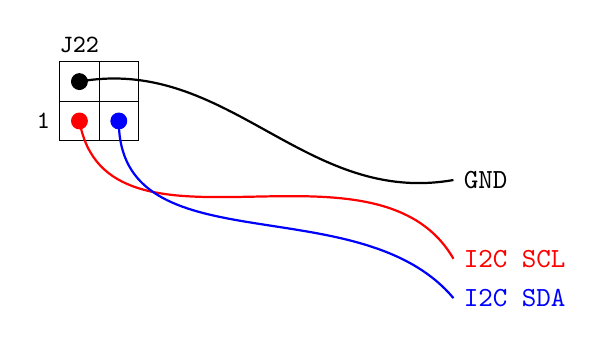
\begin{tikzpicture}
    % Pins
    \draw (0,0) rectangle (0.5,0.5);
    \draw (0.5,0) rectangle (1,0.5);
    \draw (0,-0.5) rectangle (0.5,0);
    \draw (0.5,-0.5) rectangle (1,0);

    % PCB labels
    \coordinate (A) at (0.25,0.5);
    \node at (A) [above] {\small\texttt{J22}};
    \coordinate (B) at (0,-0.25);
    \node at (B) [left] {\small\texttt{1}};

    % I2C GND
    \draw [black,fill] (0.25,0.25) circle [radius=0.1];
    \draw [thick] (0.25,0.25)
        to [out=10,in=190] (5,-1) node [right] {\texttt{GND}};

    % I2C SCL
    \draw [red,fill] (0.25,-0.25) circle [radius=0.1];
    \draw [red,thick] (0.25,-0.25) to [out=-80,in=120] (5,-2)
        node [right] {\texttt{I2C SCL}};

    % I2C SDA
    \draw [blue,fill] (0.75,-0.25) circle [radius=0.1];
    \draw [blue,thick] (0.75,-0.25) to [out=-90,in=130] (5,-2.5)
        node [right] {\texttt{I2C SDA}};
\end{tikzpicture}
\caption{Schematic for external \itwoc adapter setup.}
\label{fig:external_i2c}
\end{figure}

\input{include/hardware/gbtx_db/configure_slave_to_use_master_sca.tex}
\input{include/hardware/gbtx_db/configure_gbtx_to_use_gbt_ic.tex}
\input{include/hardware/gbtx_db/configure_gbtx_tx_rx_widebus_fec.tex}
\input{include/hardware/gbtx_db/reset_gbtx.tex}


\end{document}
